\chapter{Aktuelle Engineentwicklung}
\label{chap:engine-uebersicht}

%% Zitat:
% https://twitter.com/CompSciFact/status/527816734863265792
\epigraph{Even if your code was perfect when you released it, it still needs to be maintained because the world around it is changing.}{Unbekannt}

Spiele- und Grafikengines sind inzwischen äußerst komplexe Softwareprojekte. Früher wurden Spiele von Einzelpersonen oder kleinen Teams entwickelt, heute sind Teamstärken von über 100 Entwicklern keine Seltenheit. Komplexe Softwareprojekte erfordern neue Projektstrukturen, und dem entsprechend haben sich die Projektstrukturen im Laufe der Zeit gewandelt. Mit der Professionalisierung der Branche sind auch die Anforderungen an die Software zumindest klar definiert: Das Softwareprojekt ist langfristing angelegt, soll dem entsprechend robust und flexibel, wartbar, zugänglich und verständlich sein. Projektstrukturen sind inzwischen häufig auf kurze Iterationszyklen ausgelegt, Die dem Entwicklerteam ermöglichen sollen, auf die sich verändernde Umwelt und den neuen Anforderungen und Gegebenheiten flexibel zu reagieren.

Gerade im letzten Jahr hat sich auf dem Markt der kommerziellen Spiele- und Grafikengines einiges verändert. Die wichtigsten Entwickler von kommerziellen Engines, wie \textit{Epic Games}, \textit{Unity} oder \textit{Crytek}, haben ihre Projekte der Allgemeinheit geöffnet, während früher noch sechsstellige Beträge für den Einblick in den Quelltext zu zahlen waren. Inzwischen rufen die Entwickler direkt zur Mitarbeit an ihrer Engine auf. Das bringt für beide Seiten Vorteile. Zwar muss der beitragende Entwickler auf seine Rechte am Code verzichten\footnote{https://www.unrealengine.com/eula}, doch kann er direkten Einfluss auf Entwicklung nehmen. Und auf der anderen Seite kann das Unternehmen den Eifer der Entwickler kommerziell verwerten aber auch neue fähige Mitarbeiter rekrutieren.

Zusätzlich hat sich der Fokus der aktuellen Engines deutlich verschoben. Während noch vor ein paar Jahren die Editoren noch recht komplex zu bedienen waren und meist immer noch tiefergehende Programmierkenntnisse erforderlich waren, sind die aktuellen Editoren deutlich einsteigerfreundlicher geworden. Erste Prototypen oder einfache Spiele sind in Editoren wie dem \textit{UnrealEd} über das Blueprint genannte System ohne eigentliche Programmierkenntnisse umsetzbar. Komplexere und spezifische Blueprints werden später wieder von den Programmierern umgesetzt, die dann von Game-Designer zur Anwendung gebracht werden können.

\begin{figure}
\centering
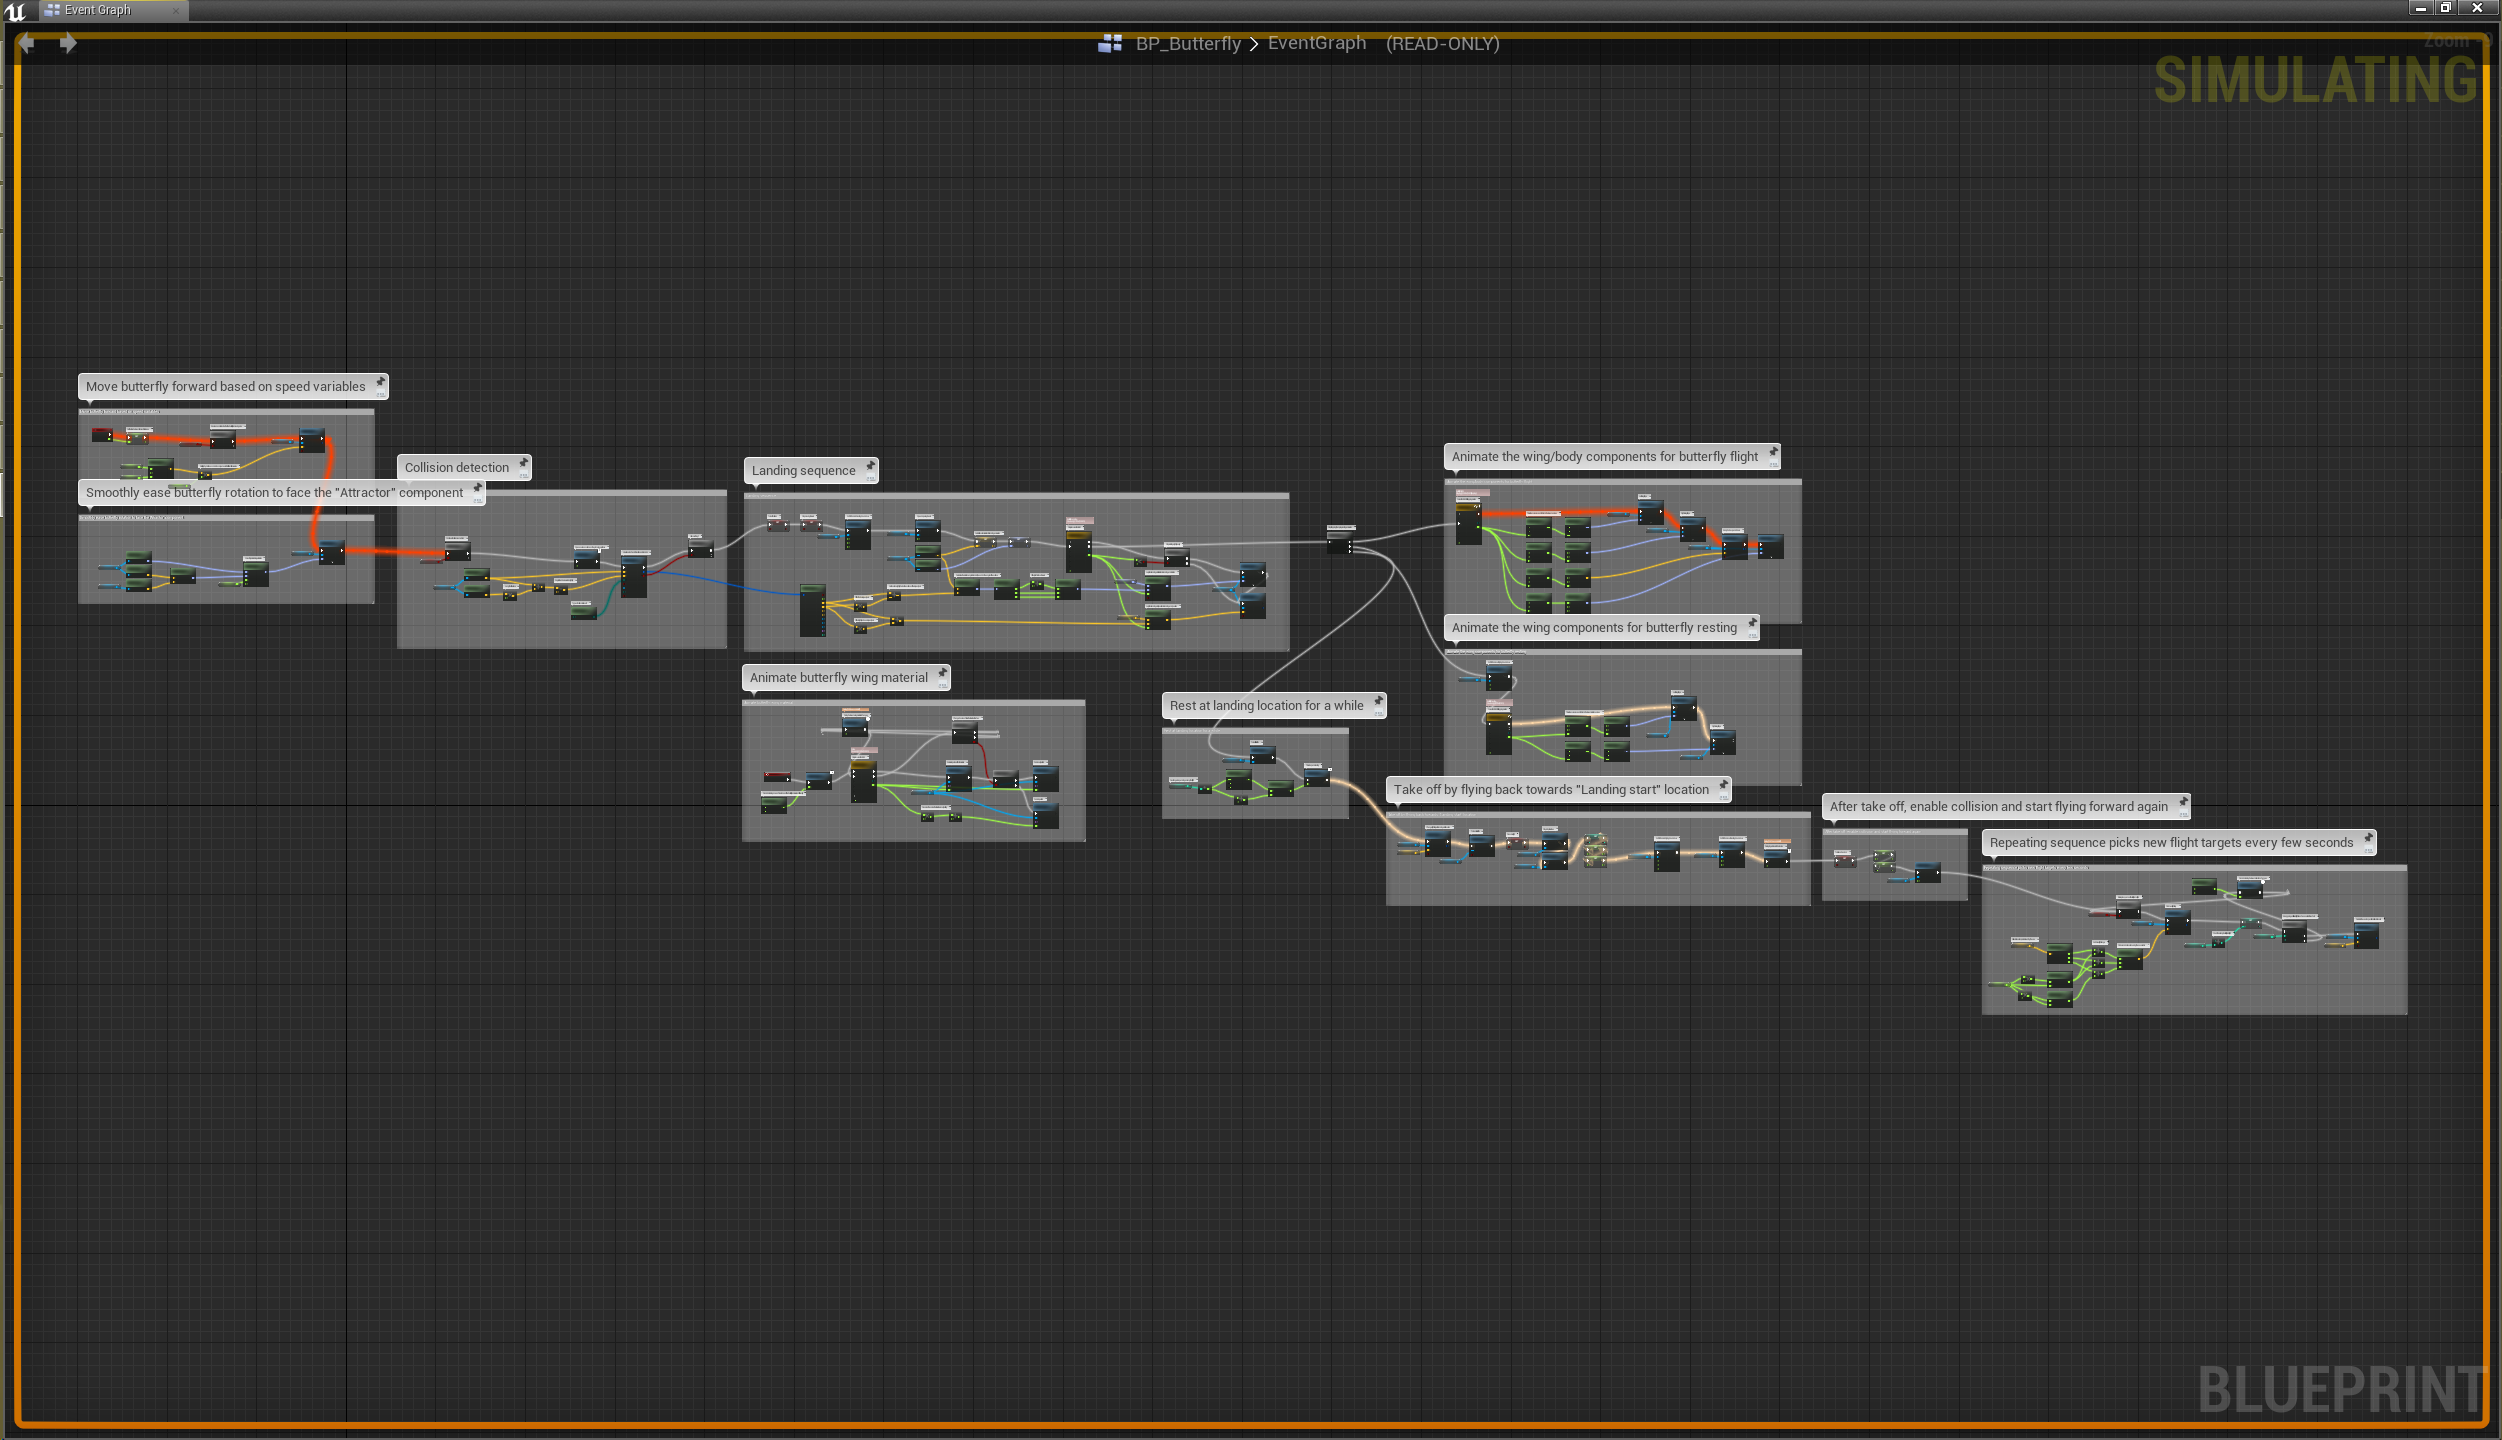
\includegraphics[width=\textwidth]{ue4-blueprint}
\caption{Unreal Engine 4 Blueprint Beispiel}
\end{figure}



\section{Grafik-Engines in Haskell}

\subsection{HGamer3D}

\textit{HGamer3D}\footnote{http://www.hgamer3d.org/} basiert auf (nich kompletten) Haskell-Bindings zu \textit{Ogre}\footnote{http://www.ogre3d.org/}. Ogre ist eine objektorientierte Open-Source Grafik-Engine geschrieben in C++. Ohne weiter auf die Fähigkeiten der Ogre Engine einzugehen, stellt sich oft die Adaptierunung von imperativen Bibliotheken auf funktionale Konzepte als aufwändig und nicht immer optimal heraus. Insbesondere das Erzeugen von Bindings zu komplexen \acsp{API}s ist immer noch eine hohe Hürde.

Auch wenn Ogre als Framework viele Strukturen und Lösungsansätze für gängige Probleme in der 3D Computergrafik und Spieleprogrammierung bereitstellt, ließen sich viele Ansätze auch direkt funktional umsetzen, ohne große und schwerfällige \acsp{API}s zähmen zu müssen.

Zum Beispiel verfolgen beide Welten zum Teil gänzlich andere Grundprinzipien. So sind Daten in Haskell prinzipiell unveränderlich während in C++ Daten prinzipiell veränderlich sind. Haskell erlaubt unter anderem deswegen andere Ansätze der Nebenläufigkeit (Concurrency). Speziell Nebenläufigkeiten stellen immer noch in komplexen Softwareprojekten eine große Hürde dar. Die Adaption einer C++-Biblithek kann das Ausnutzen vieler Vorteile von Haskell behindern (weitere Ausführungen in \fref{sec:warum-haskell}).

Zusätzlich entstehen durch Bindings zu externen Biblitheken neue Abhängigkeiten, die oft eine Anpassung der Tool-Chain erfordern, da sie nicht in das bestehende Ökosystem passen. Dies erhöht die Komplexität des Gesamtsystems. Die Erfahrung des Autos hat gezeigt, dass eigentlich jedes externes Binding früher oder später zu Komplikationen führt, spätestens dann, wenn die Anwendung die Entwicklungsumgebung verlässt. Doch lässt sich nicht jede Abhhängigkeit zu anderen Sprachen vermeiden. Insbesondere in der Grafikprogrammierung mit OpenGL werden die eigentlichen Bindings zu der OpenGL-API benötigt. Zusätzlich muss noch ein platformabhängiger Render-Kontext erzeugt werden.

Meinung des Autors: Es sollten möglichst wenige Fremdabhängigkeiten aus anderen Sprachen genutzt werden, leider ist dies nicht immer möglich (Weitere Ausführungen in \fref{sec:probleme-haskell}). Mit den Ogre Bindings wird die eine komplexe schwer funktional bezwingbare \acs{API} (z.B. OpenGL) mit einer anderen ersetzt.

\subsection{LambdaCube 3D}

\textit{LambdaCube 3D}\footnote{https://lambdacube3d.wordpress.com/} ist eine in Haskell definierte und beeindruckende \ac{DSL}, die es erlaubt Grafikanwendungen bis hin zum Shader komplett in Haskell zu formulieren. Da OpenGL eine komplexe und übersichtliche \acs{API} ist, ist die \ac{DSL} entsprechend komplex und unübersichtlich. Zusätzlich basiert das OpenGL Backend noch auf der Version 3.2. Die Dokumentation beschränkt sich auf den Blog und eine handvoll Beispielen, so dass es schwer ist einen Zugang zu der DSL zu erhalten.

Aber generell stellt sich die bei OpenGL die Frage, wie sinnvoll es ist die komplexe \acs{API} in einer anderen Sprache komplett abzubilden, mit all ihren erlaubten und nicht erlaubten Zuständen, die zusätzlich noch treiberspezifisch sind. Hinzu kommen diverse Erweiterungen, die oft Verhaltensweisen der \acs{API} massiv beeinflussen.

Die persönliche Einschätzung des Autors ist, dass sich OpenGL nicht in einem vertretbaren Aufwand komplett abbilden lässt. Der Aufwand wäre ungefähr mit dem vergleichbar, den Grafikkartenhersteller bei der Implementierung ihrer Grafikkartentreiber betreiben (weitere Ausführungen in \fref{chap:modern-opengl}). Deswegen sollte eine Auswahl der direkten OpenGL Bindings getroffen werden um sie punktuell in funktionale Konzepte zu gießen.

% \subsection{Elm}

% \subsection{Gloss}
% Gloss (2d) ist ein schönes Beispiel dafür wie sich mit einem OpenGL backend und mit der konzentration auf das wesentliche eine klare funktionale api schaffen lässt die einfach anzuwenden ist.
